% Flushed left equation
%\documentclass[a4paper,fleqn,usenatbib]{aspdoc}
% Centered equation
\documentclass[a4paper,usenatbib]{aspdoc}
%\documentclass[]{article}
\usepackage{newtxtext,newtxmath}
\usepackage{ae,aecompl}
\usepackage{graphicx}	% Including figure files
\usepackage{amsmath}	% Advanced maths commands
\usepackage{amssymb}	% Extra maths symbols
\usepackage{lipsum}
\usepackage{float}
\usepackage{multirow}
\usepackage{booktabs}
\usepackage{geometry}
\geometry{left=25mm,right=25mm,top=25mm,bottom=25mm}

\newcounter{simplecount}
\setcounter{simplecount}{0}
\renewcommand{\theequation}{\arabic{simplecount}}
\newcommand{\owncount}{\refstepcounter{simplecount}}


% Title
\title[]{TRA: Der Bipolartransistor und die Emitterschaltung}

% The list of authors
\author[]{
    Riedel Lisa, Wegmann Peter
    \newauthor
    \,Gruppe 6
    %\\
    %$^{1}$Fakultät für Physik, Technische Universität München\\
}

% Don't change these lines
\begin{document}
    \label{firstpage}
    \pagerange{\pageref{firstpage}--\pageref{lastpage}}
    \maketitle
    
    
    
    % Body
    \section{Einleitung} 
        In diesem Versuch wird ein Bipolartransistor in eine Schaltung eingebaut und diese genauer untersucht. Bei der resultierenden Schaltung handelt es sich um eine Emitterschatung. Bei einer Emmiterschaltung handelt es sich um einen Verstärker, der bei einer kleinen, angelegten Spannung eine große Verstärkerung bewirken kann. \\
        \textbf{Vorüberlegung 1:} Sollten Widerstände und Kapazitäten innerhalb der Schaltung gemessen werden, wird sowohl der komplette Schaltkreis miteinbezogen als auch eine zusätzliche Spannung durch das Multimeter angelegt. Dies würde zu verfälschten Ergebnissen führen. Daher sollten Komponenten immer isoliert betrachtet werden. Bei dem Versuch wurde innerhalb der Schaltung -1.33k$\Omega$ gemessen, außerhalb 7.13 k$\Omega$. Ein negativer Wert für den Widerstand ist unphysikalisch. Diese Methode ist daher aufgrund oben genannter Fehler nicht geeignet. \\
        \textbf{Vorüberlegung 2:} Es soll die Gleichung
        
        \begin{equation}
            \owncount
            \begin{pmatrix}
                i_b \\
                i_c
            \end{pmatrix}
                =
            \begin{pmatrix}
                \frac{1}{r_{BE}} & 0 \\
                S & \frac{1}{r_{CE}}
            \end{pmatrix}
            \begin{pmatrix}
                u_{BE} \\
                u_{CE}
            \end{pmatrix} \\
        \end{equation}
        in h-Parameter überführt werden. Das Gleichungssystem sieht dann wie folgt aus.
        \begin{equation}
            \owncount
            \begin{pmatrix}
                u_{BE} \\
                i_c
            \end{pmatrix}
                 =
            \begin{pmatrix}
                r_{BE} & 0 \\
                S r_{BE} & \frac{1}{r_{CE}}
            \end{pmatrix}
            \begin{pmatrix}
                i_b \\
                u_{CE}
            \end{pmatrix}
        \end{equation} \\
        Die Beziehung zwischen der Steilheit S und der differentiellen Stromverstärkung $\beta$ sieht wie folgt aus. 
        \begin{equation}
            \owncount
            S = \frac{\partial I_C}{\partial U_{BE}} | U_{CE} , 
            \beta = \frac{\partial I_C}{\partial I_B} | U_{CE} 
            \Rightarrow S = \beta \frac{\partial I_B}{\partial U_{BE}} = \frac{\beta}{r_{BE}}
       \end{equation}
        
  
    
    \section{Verwendete Methoden}
        Die Emitterschaltung dient der Verstärkung von elektrischen Signalen im niederfrequenten Bereich. Der eingebaute Bipolartransistor ist Temperaturabhängig. Damit sich der vorher eingestellte Arbeitspunkt deswegen nicht verändert, wird die Emitterschaltung mit Arbeitspunktstabilisierung durch Stromgegenkopplung betrieben.
        Um die Messergebnisse auszuwerten, werden folgende Formeln aus der Anleitung entnommen (\cite{anleitung}). \\ 
        Der Differentielle Widerstand $r_{BE}$ und $r_{CE}$, sowie die Steilheit S berechnet sich aus dem Ebers-Moll-Modell. Ebenso kann über die exponentielle Abhängigkeit des Basisstorms die Temperatur des Transistors angegeben werden. 
        \begin{equation}
            \owncount
            \frac{1}{r_{\mathrm{BE}}}=\frac{\partial I_{\mathrm{B}}}{\partial U_{\mathrm{BE}}} | U_{\mathrm{CE}}
            \Rightarrow r_{\mathrm{BE}} = (\frac{\partial I_{\mathrm{B}}}{\partial U_{\mathrm{BE}}} | U_{\mathrm{CE}})^{-1}
            \label{eq:rbe}
        \end{equation}
        
        \begin{equation}
            \owncount
            \frac{1}{r_{\mathrm{CE}}}=\frac{\partial I_{\mathrm{C}}}{\partial U_{\mathrm{CE}}} | U_{\mathrm{BE}}
            \Rightarrow r_{\mathrm{CE}} = (\frac{\partial I_{\mathrm{C}}}{\partial U_{\mathrm{CE}}} | U_{\mathrm{BE}})^{-1}
            \label{eq:rce}
        \end{equation}
        
        \begin{equation}
            \owncount
            S=\left.\frac{\partial I_{\mathrm{C}}}{\partial U_{\mathrm{BE}}}\right|_{U_{\mathrm{CE}}}=\frac{q I_{\mathrm{C}}}{k_{\mathrm{B}} T}
            \label{eq:T}
        \end{equation}
        
        \begin{equation}
            \owncount
            I_B \propto \exp{\frac{qU_{BE}}{k_BT}}
            \label{eq:Texp}
        \end{equation}
        
        \noindent Im späterem Verlauf soll die Spannungsverstärkung der Emitterschaltung berechnet werden. Hierbei ist zu beachten, ob ein Kondensator angeschlossen ist oder nicht. 
        \begin{equation}
            \owncount
            A = \frac{dU_a}{dU_e} = -S(R_C\parallel r_{CE}\parallel R_L)
            \label{eq:A}
        \end{equation}
        
        \begin{equation}
            \owncount
            A \approx -\frac{R_C \parallel R_L}{R_E}
            \label{eq:Aapprox}
        \end{equation}
        
        \noindent Zudem wird in der letzten Aufgabe die Impetanz bei einem einfachen Zweitor als Hoch - oder Tiefpassfilter gemessen. Hierfür wird die folgende Matrix benötigt.
        
        \begin{equation}
            %\owncount
            \begin{pmatrix}
                \underline{I}_e \\
                \underline{I}_a
            \end{pmatrix}
                =
            \begin{pmatrix}
                \frac{1}{\underline{Z}_1} & -\frac{1}{\underline{Z}_1} \\
                -\frac{1}{\underline{Z}_1} & \frac{1}{\underline{Z}_1} + \frac{1}{\underline{Z}_2}
            \end{pmatrix}
            \begin{pmatrix}
                \underline{U}_e \\
                \underline{U}_a
            \end{pmatrix} \\
        \end{equation}
    

    
    \section{Experimentelles Vorgehen}
    In dem Versuch wurden mit einem digitalen Multimeter und einem Oszilloskop Messungen durchgeführt. Beim Oszilloskop war der Faktor 10 für den Tastteiler eingestellt. 
    
    \noindent Bei der Messerung der Verstärkung in der Emittenschaltung wurden bei allen drei Konstellationen jeweils $u_e$ und $u_a$ bei 10 Messpunkten gemessen. Der Widerstand $R_C$ wurde von 1 k$\Omega$ bis 10 k$\Omega$ variiert. Die Messwerte wurden vom Oszilloskop abgelesen, $R_C$ wurde mit Hilfe des Multimeters eingestellt.
    
    \noindent Beim Messen des Frequenzganges wurde die Frequenz von 6Hz bis 250kHz variiert. Dabei wurde wieder $u_e$ und $u_a$ vom Oszilloskop abgelesen, und mit Hilfe des Cursors $\delta t$ bestimmt. Insgesamt wurden 26 Messpunkte abgenommen. Da die Kurve ein Plateau aufweist, wurde in dessen Nähe wenig Messwerte erhoben.
    
    \noindent Bei der Messung der Eingangs- und Ausgangkennlinie wurde das Multimeter verwendet. Eines wurde zur Messung des elektrischen Stroms und das andere zur Messung der Spannung verwendet. Über ein zusätzliches Multimeter konnte die andere Spannung überprüft und angepasst werden, da sie für die jeweilige Kennlinie konstant gehalten werden musste. Für die Eingangskennlinie wurden 15 Datenpunkte erhoben. Bei geringer Spannung wurden einige wenige Datenpunkte aufgezeichnet, da der Strom sehr klein war. Bei hoher Spannung wurden mehr Datenpunkte aufgezeichnet, da der Strom rapide anstieg. Bei der Ausgangskennlinie wurden 10 Punkte gemessen, relativ viele bei kleiner Spannung, aufgrund der rapiden Stromzunahme, und wenige bei hoher Spannung, da der Strom annähernd konstant geblieben ist.
    
    
        % TODO Beschreiben wie gemessen wurde
        % TODO Anzahl der gemessenen Datenpunkte beschreiben
        % TODO Welche Aparaturen und Geräte wurden verwendet
        % TODO Nennung wichtiger Einstellungen
    
    
    \section{Ergebnisse}
        % TODO Angabe der Messergebnisse (Mittelwert) mit Unsicherheiten
        % TODO Unsicherheiten diskutieren
        % TODO Beschreibung der Graphen und Tabellen
        % TODO Vergleich von Ergebnisse die auf unterschiedliche Weise berechnet wurden
        % TODO Gründe für Abweichungen anführen
        % TODO Ist das Resultat realistisch und was sagt es aus
        
        \subsection{Kleinsignalgrößen}
            % 1
            Zur Bestimmung der Kleinsignalgrößen des verwendeten Transistors müssen dessen Kennlinien ermittelt werden. Hierzu wurde die Eingangskennlinie, in welcher $I_B$ als Funktion von $U_{BE}$ bei konstantem $U_{CE}$ aufgetragen wird, und die Ausgangskennlinie, in welcher $I_C$ als Funktion von $U_{CE}$ bei konstantem U BE aufgetragen wird, erstellt. Dazu wurde für $U_{CE}$ = 5,32V und $U_{BE}$ = 560mV gewählt, welche den Werten beim Einstellen des Arbeitspunktes für $R_C$ = 5 k$\Omega$ entsprechen.
            
            \noindent Im folgenden werden die Kleinsignalgrößen $r_{\mathrm{BE}}, r_{\mathrm{CE}}, T, S$ berechnet. Hierbei folgt eine genauere Beschreibung der berechneten Größen im jeweiligen Abschnitt.
            
            \begin{figure*}
                \centering
                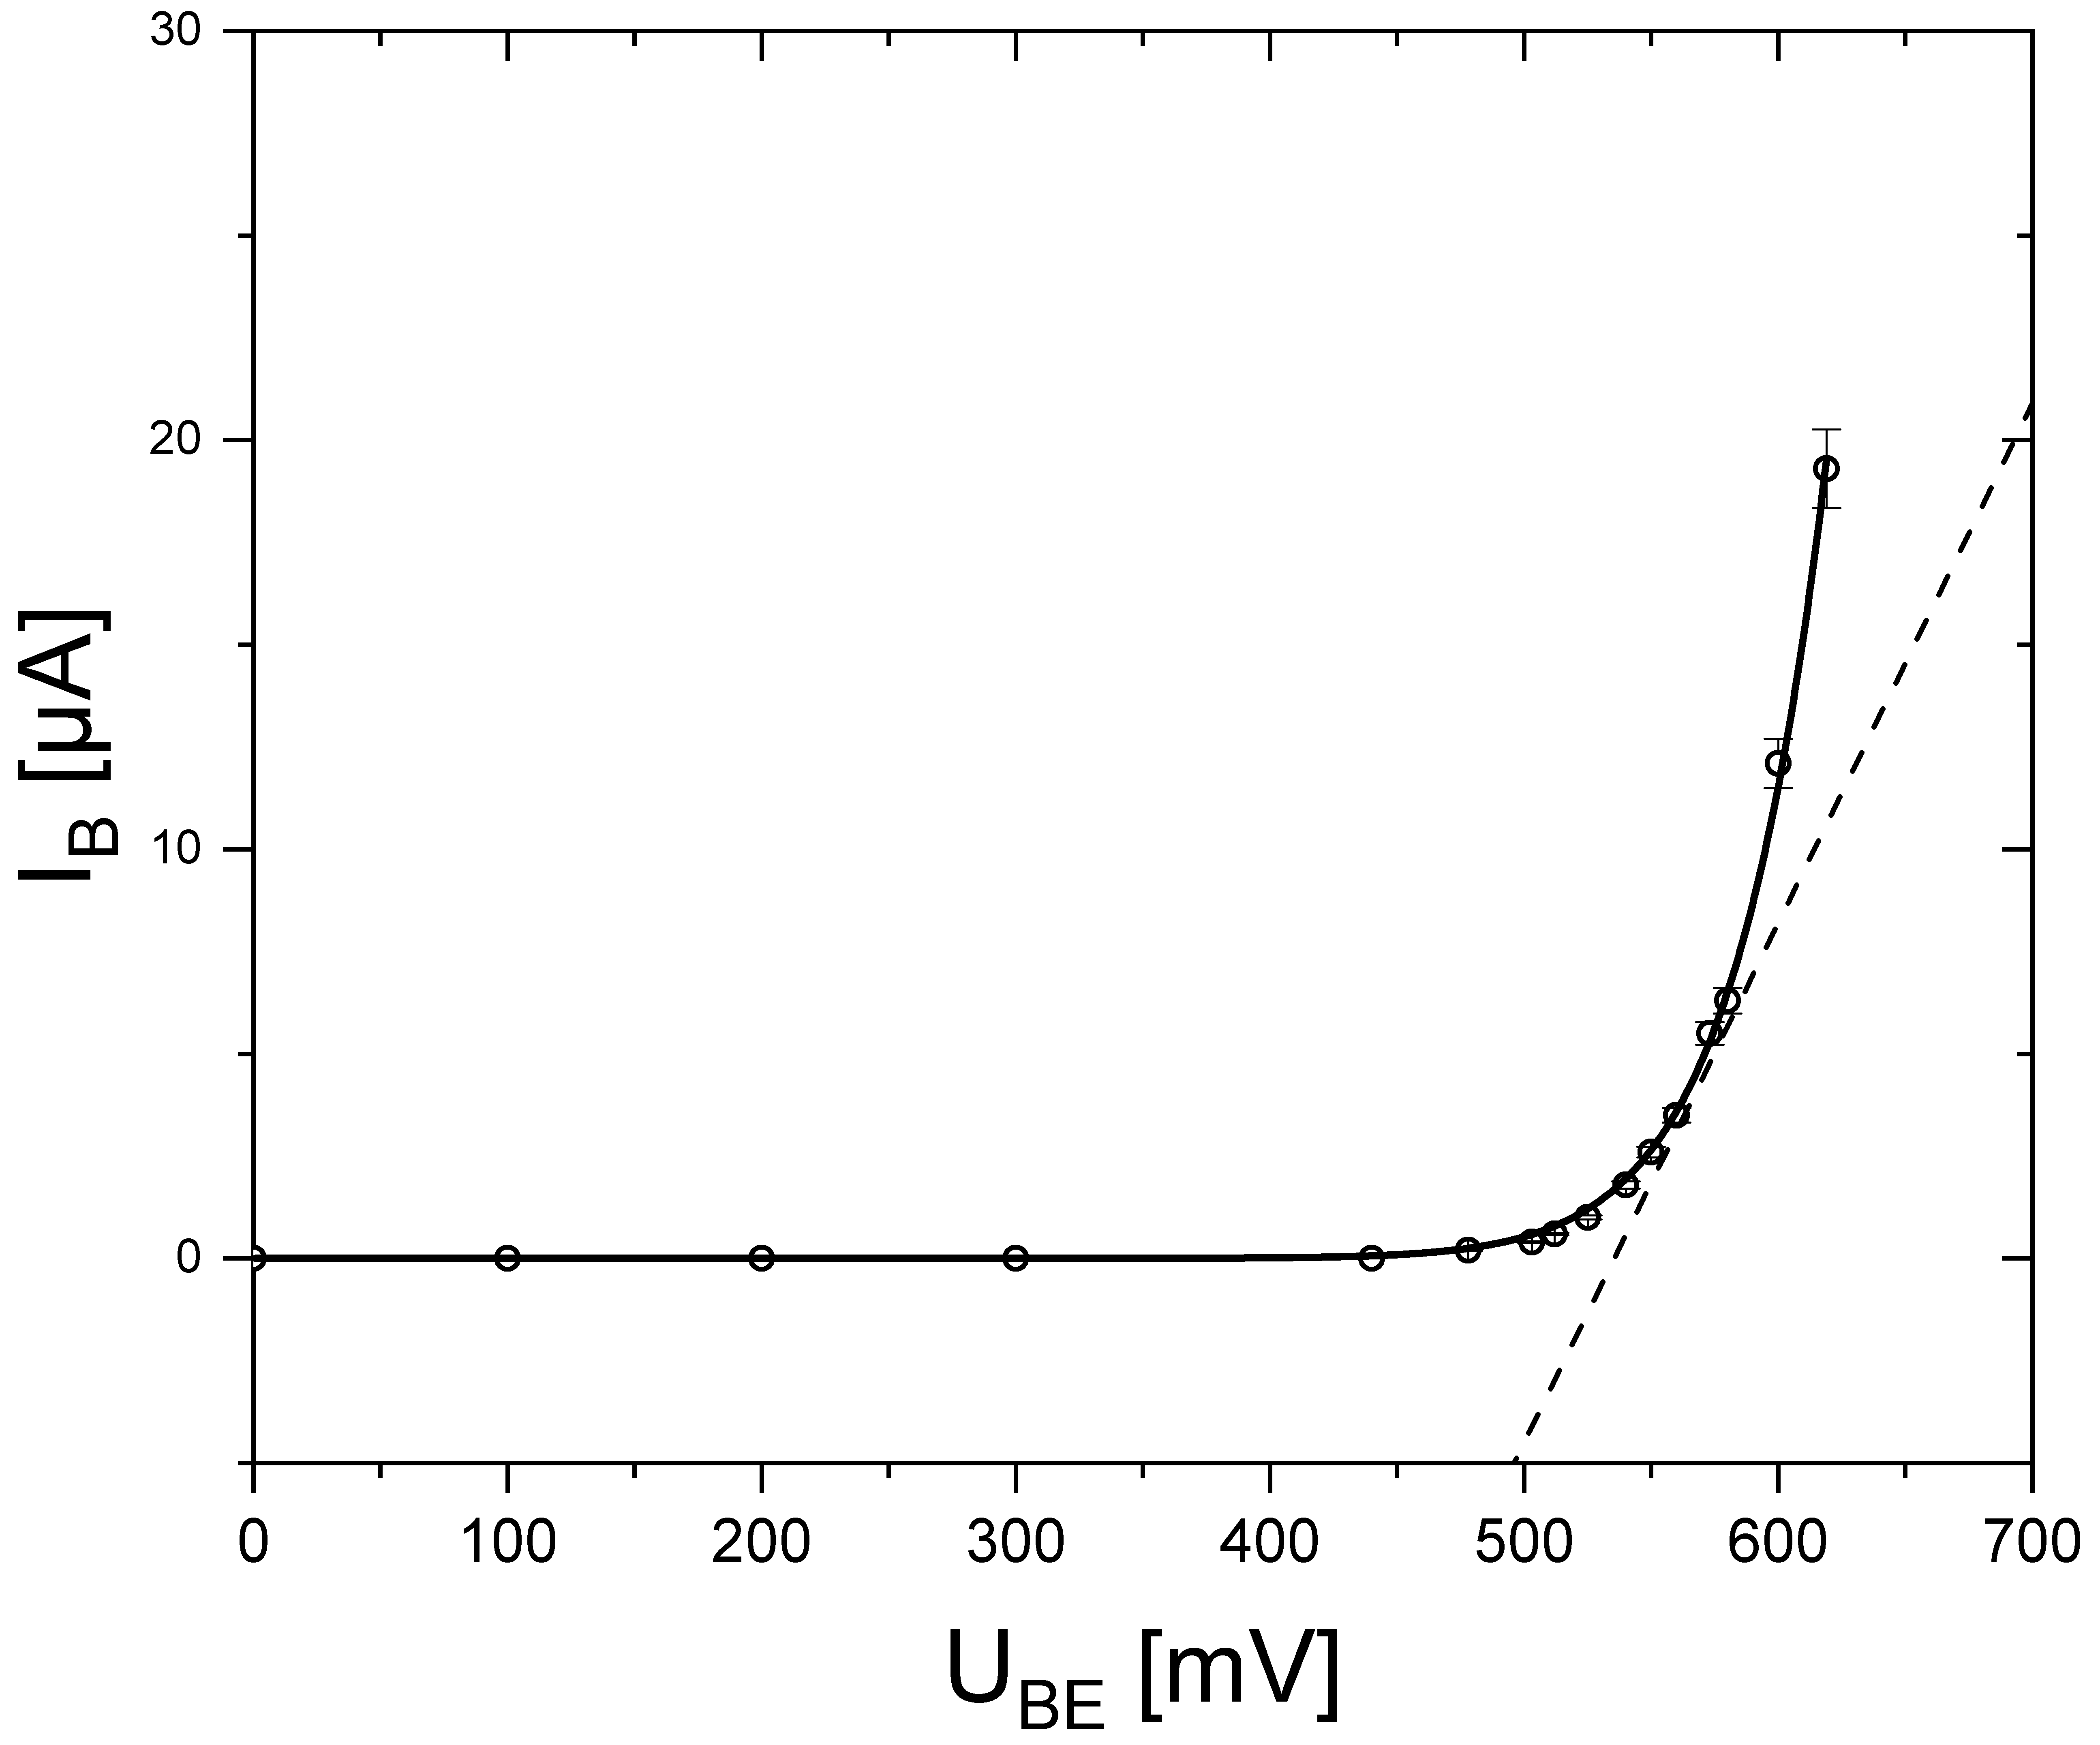
\includegraphics[width=78mm]{graphs/Kennlinie11.png}
                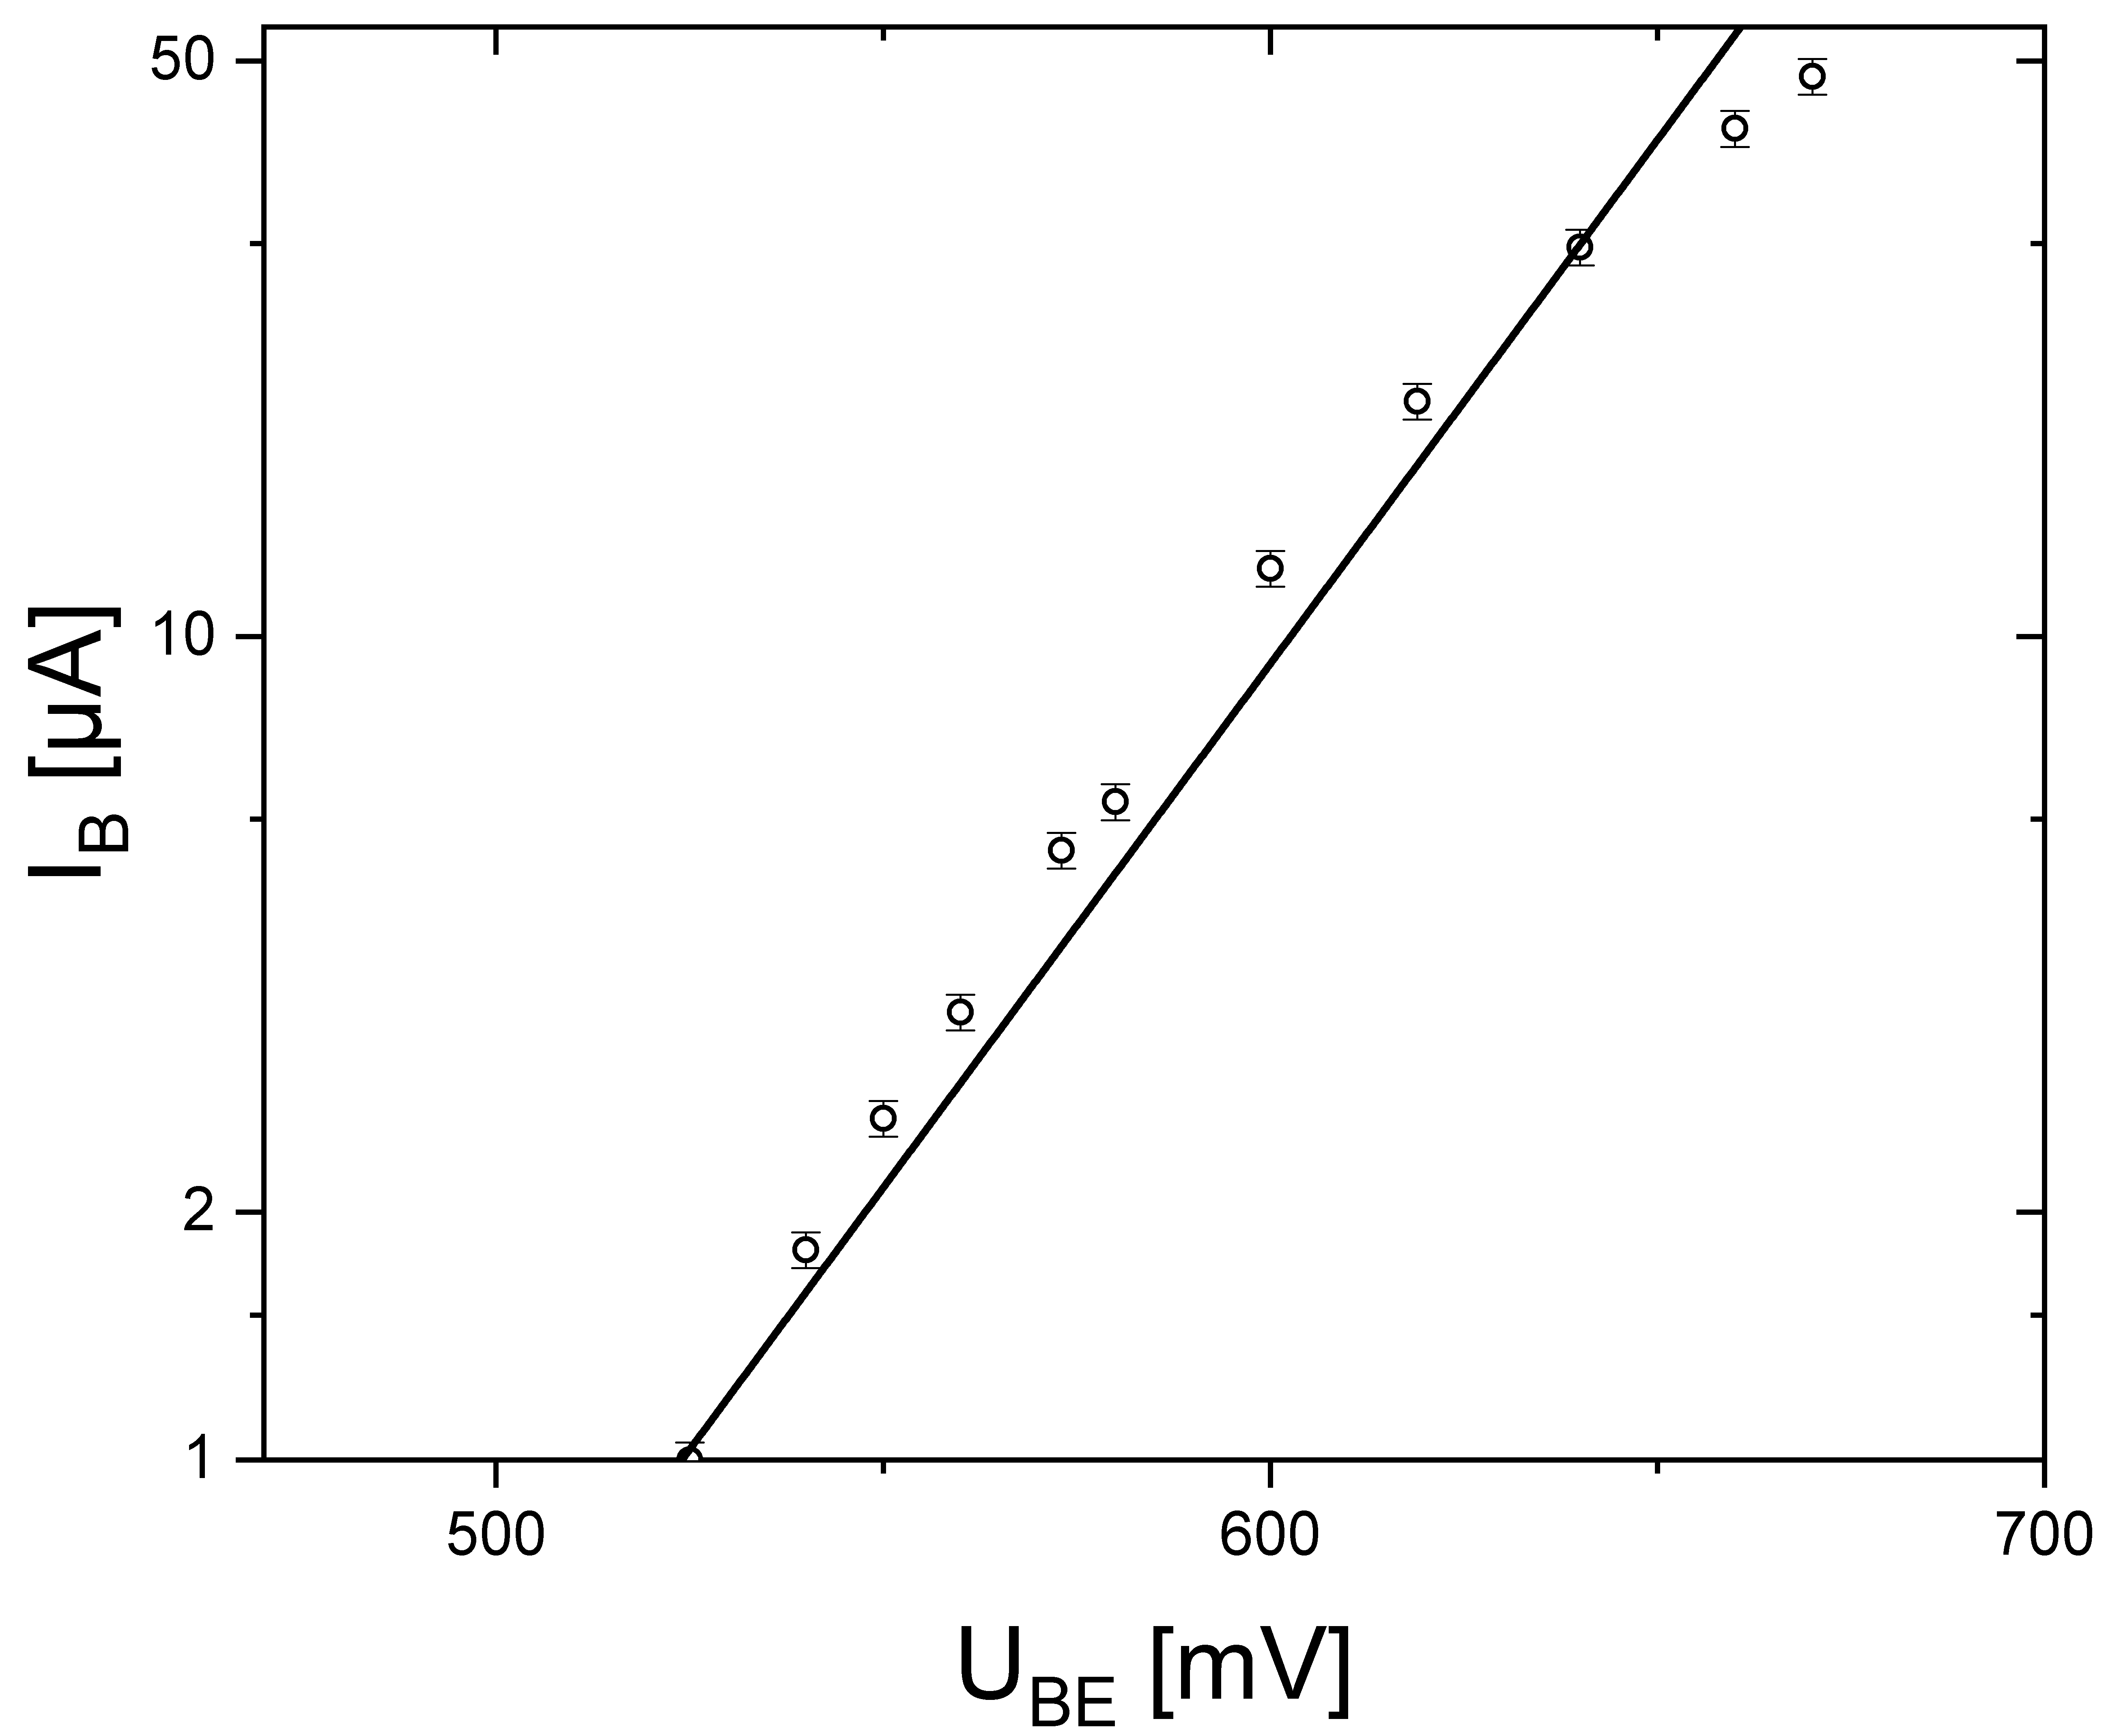
\includegraphics[width=78mm]{graphs/Kennlinie11EXP.png}
                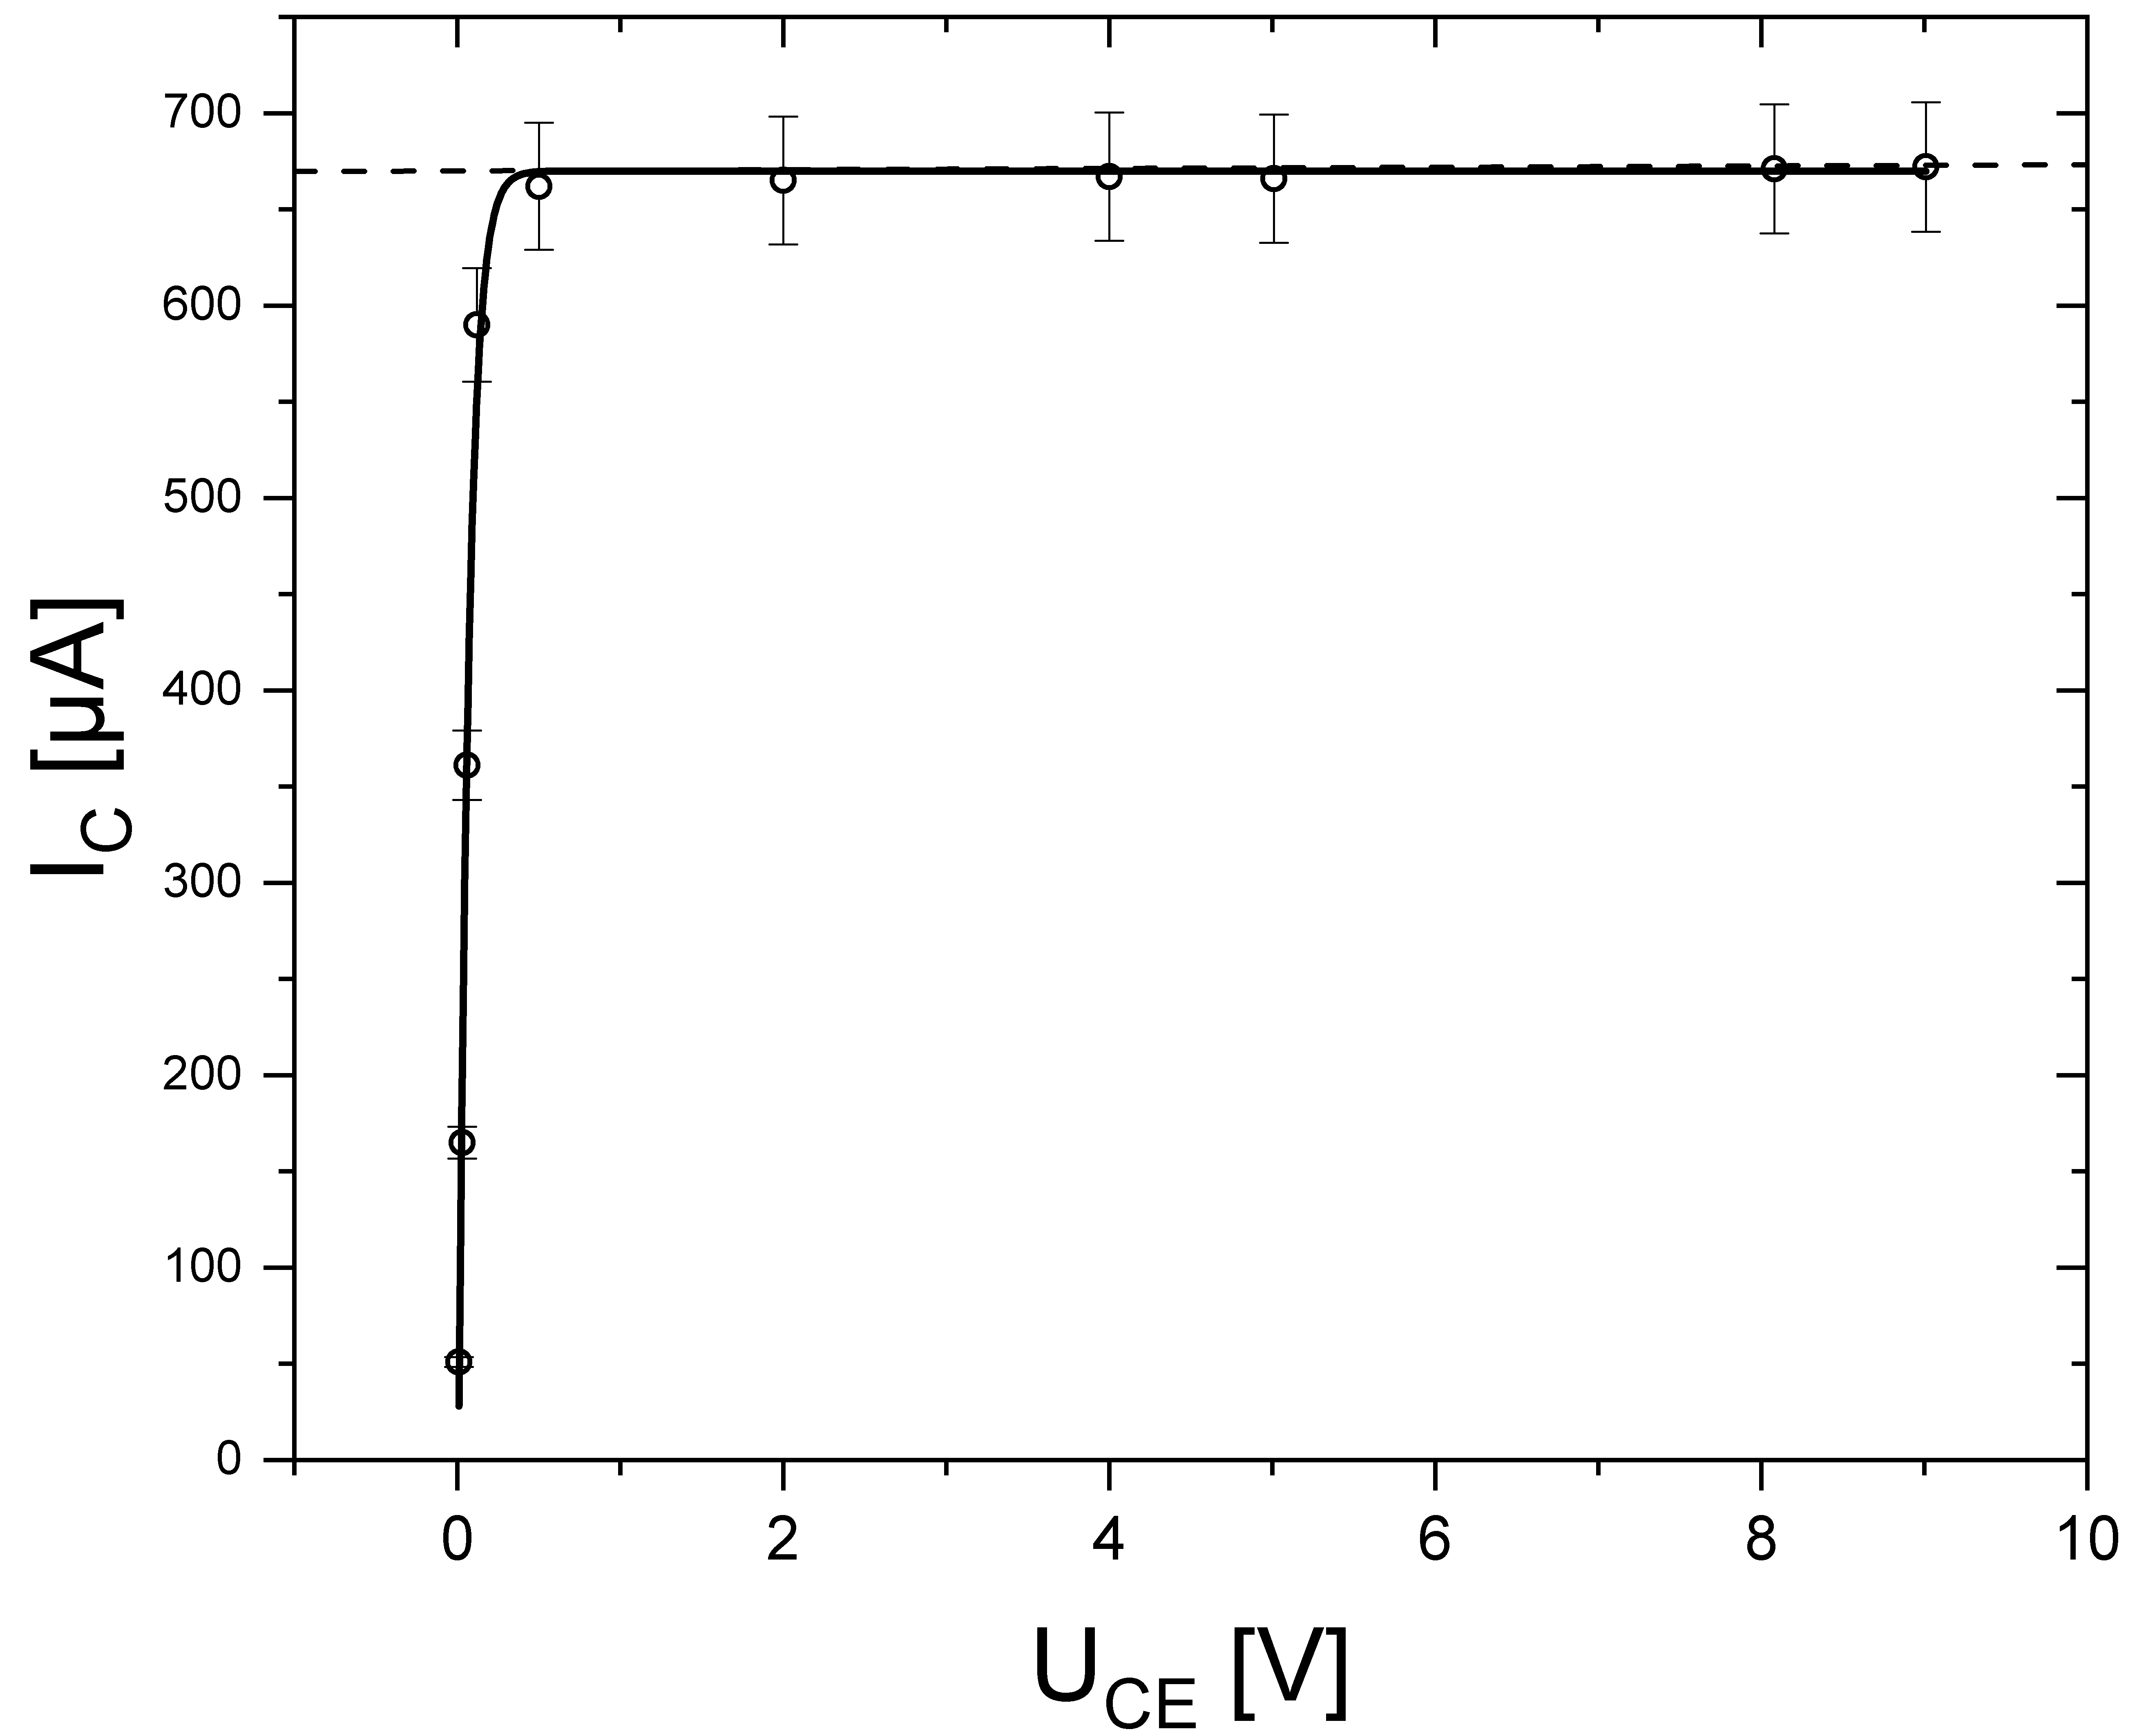
\includegraphics[width=78mm]{graphs/Kennlinie12.png}
                \caption{Kennlinien des Transistors unter Verwendung von Schaltung 13 (\cite{anleitung}). Bei der ersten Kennlinie handelt es sich um die Eingangskennlinie $I_{\mathrm{B}}=\left.f\left(U_{\mathrm{BE}}\right)\right|_{U_{\mathrm{CE}}}$, wobei $U_{\mathrm{CE}}$ konstant gehalten wurde. Der zweite Graph stellt ein Exponential/Linear fitting der ersten Kennlinie dar. Bei dem letzten Graph handelt es sich um die Ausgangskennlinie $I_{\mathrm{C}}=\left.f\left(U_{\mathrm{CE}}\right)\right|_{U_{\mathrm{BE}}}$, wobei $U_{\mathrm{BE}}$ konstant gehalten wurde.}
                \label{fig:kennlinie}
            \end{figure*}
            
            % 2
        \subsubsection{Differentielle Widerstand der Basis-Emitterschaltung}
                Der differentielle Widerstand der Basis-Emitterschaltung kann über die Eingangskennlinie \ref{fig:kennlinie} berechnen werden. Die Berechnung des differentiellen Widerstand $r_{\mathrm{BE}}$  erfolgt durch Formel \ref{eq:rbe}. 
                
                \noindent Hierfür ergibt sich ein Wert von $\mathbf{r_{\mathrm{BE}} = 7,87k\Omega}$.
                
                \noindent Hierbei wurde für $\frac{\partial I_{\mathrm{B}}}{\partial U_{\mathrm{BE}}} | U_{\mathrm{CE}}$ die Steigung der Tangente am Arbeitungspunkt in Grafik \ref{fig:kennlinie} gemessen und verwendet. Diese Beträgt $0,127 \cdot 10^{-3} \frac{1}{\Omega}$. Der Arbeitspunkt wurde hierfür bei $U_{\mathrm{BE}}=560$mV gewählt.
                
                \noindent Dieser Wert erscheint sehr groß, da aber in der gemessenen Schaltung keine $R_E$ Widerstand eingebaut worden ist, wurde dabei der Widerstand des Bipolartransistors gemessen, der nach Angabe sehr hoch ist.
            
        \subsubsection{Arbeitstemperatur}
            Für die Berechnung der Arbeitstemperatur $T$ wird die Beziehung \ref{eq:Texp} verwendet. Auffällig ist, dass sich $I_B$ propotional zur Exponentialfunktion verhält. Stellt man dieses Verhältnis nun um, so erhält man für $I_B$ den Ausdruck 
            \begin{equation}
                \owncount
                \log(I_B) = \frac{eU_{BE}}{k_BT}
            \end{equation} 
            
            \noindent Die Steigung dieser neuen Kennlinie in Abhängigkeit von $U_{BE}$ lässt sich aus der Grafik \ref{fig:kennlinie} herauslesen und damit anschließend den Wert der Temperatur berechnen.\\
            Für die Steigung erhält man folgende Beziehung: 
            \begin{equation}
                \owncount
                \frac{1}{t_1} = \frac{e}{k_BT}
                \Rightarrow T = \frac{et_1}{k_B}
            \end{equation}
            In diesen Formeln ist $t_1 = 29,3 \cdot 10^{-3}$ die Steigung des exponentiellen Fittings und $e$ die Elektronenladung. Für die Temperatur erhält man daraus den Wert $\mathbf{ T = (339,17 \pm 3,49) K} $. \\
            
        % 3
        \subsubsection{Steilheit}\label{subsec:Steil}
            Die Steilheit S des Transistors ist ein Maß für die Änderung des Kollektorstroms $I_C$ bei Veränderungen der Basis-Emitterspannung $U_{BE}$. Man bezieht sisch auf die Formel \ref{eq:T}. Der Wert für $I_C$ wurde bei den Widerständen $R_C = 1k\Omega , 5k\Omega$ und $10 k\Omega$ gemessen und war annähernd gleich. Für die weitere Rechnung wurde mit dem Mittelwert 0.64 mA gerechnet. Daher kann die Steilheit S für das gesamte System über die Formel \ref{eq:T} berechnet werden. 
            $\mathbf{S = (2,16 \pm 0,21) \cdot 10^{-2} \frac{1}{\Omega}}$ \\
            
            
            % 4
        \subsubsection{Differentielle Widerstand der Kollektor-Emitterschaltung}
            Der differentielle Widerstand $r_{CE}$ lässt sich aus der Ausgangskennlinie \ref{fig:kennlinie} berechnen. Die Berechnung $r_{\mathrm{CE}}$ wird durch Formel \ref{eq:rce} durchgeführt. Auch hier wird für $\frac{\partial I_{\mathrm{C}}}{\partial U_{\mathrm{CE}}} | U_{\mathrm{BE}}$ die Steigung der Tangente am Arbeitspunkt berechnet und verwendet. Bei dem verwendeten Arbeitungspunkt handelt es sich um $U_{\mathrm{CE}} = 5.36$V. Daraus erhält man den Wert $\mathbf{r_{CE} = 3,13 \cdot 10^{6} M\Omega}$.\\
            Dieser Wert erscheint sinnvoll zu sein, da der gemessene Widerstand des Bipolartransistor, wie in der Angabe angemerkt, sehr hoch ist. Dieser hohe Wert ermöglicht somit eine Verstärkung. \\
            
            
    
        \subsection{Verstärkung}\label{subsec:Versärkung}
            Im folgenden gilt es die Verstärkung der drei verschiedenen Anordnungen, wie in Grafik \ref{fig:verstärkung} sichtbar, sowohl theoretisch als auch aus den gemessenen Werten der Amplituden des Eingangssignal $u_a$ und Ausgangssignal $u_e$ zu berechnen.\\
            In Grafik \ref{fig:verstärkung} ist die Verstärkung der Emitterschaltung unter verschiedenen Konfigurationen sichtbar. Hierbei ist die Wichtigkeit des Kondensators $C_E$ gut erkennbar. Zu den gemessenen Werten, lassen sich die Verstärkungen unter den Konfigurationen durch Formel \ref{eq:A} und Formel \ref{eq:Aapprox} berechnen. 
            
            % 1
            \begin{figure*}
                \centering
                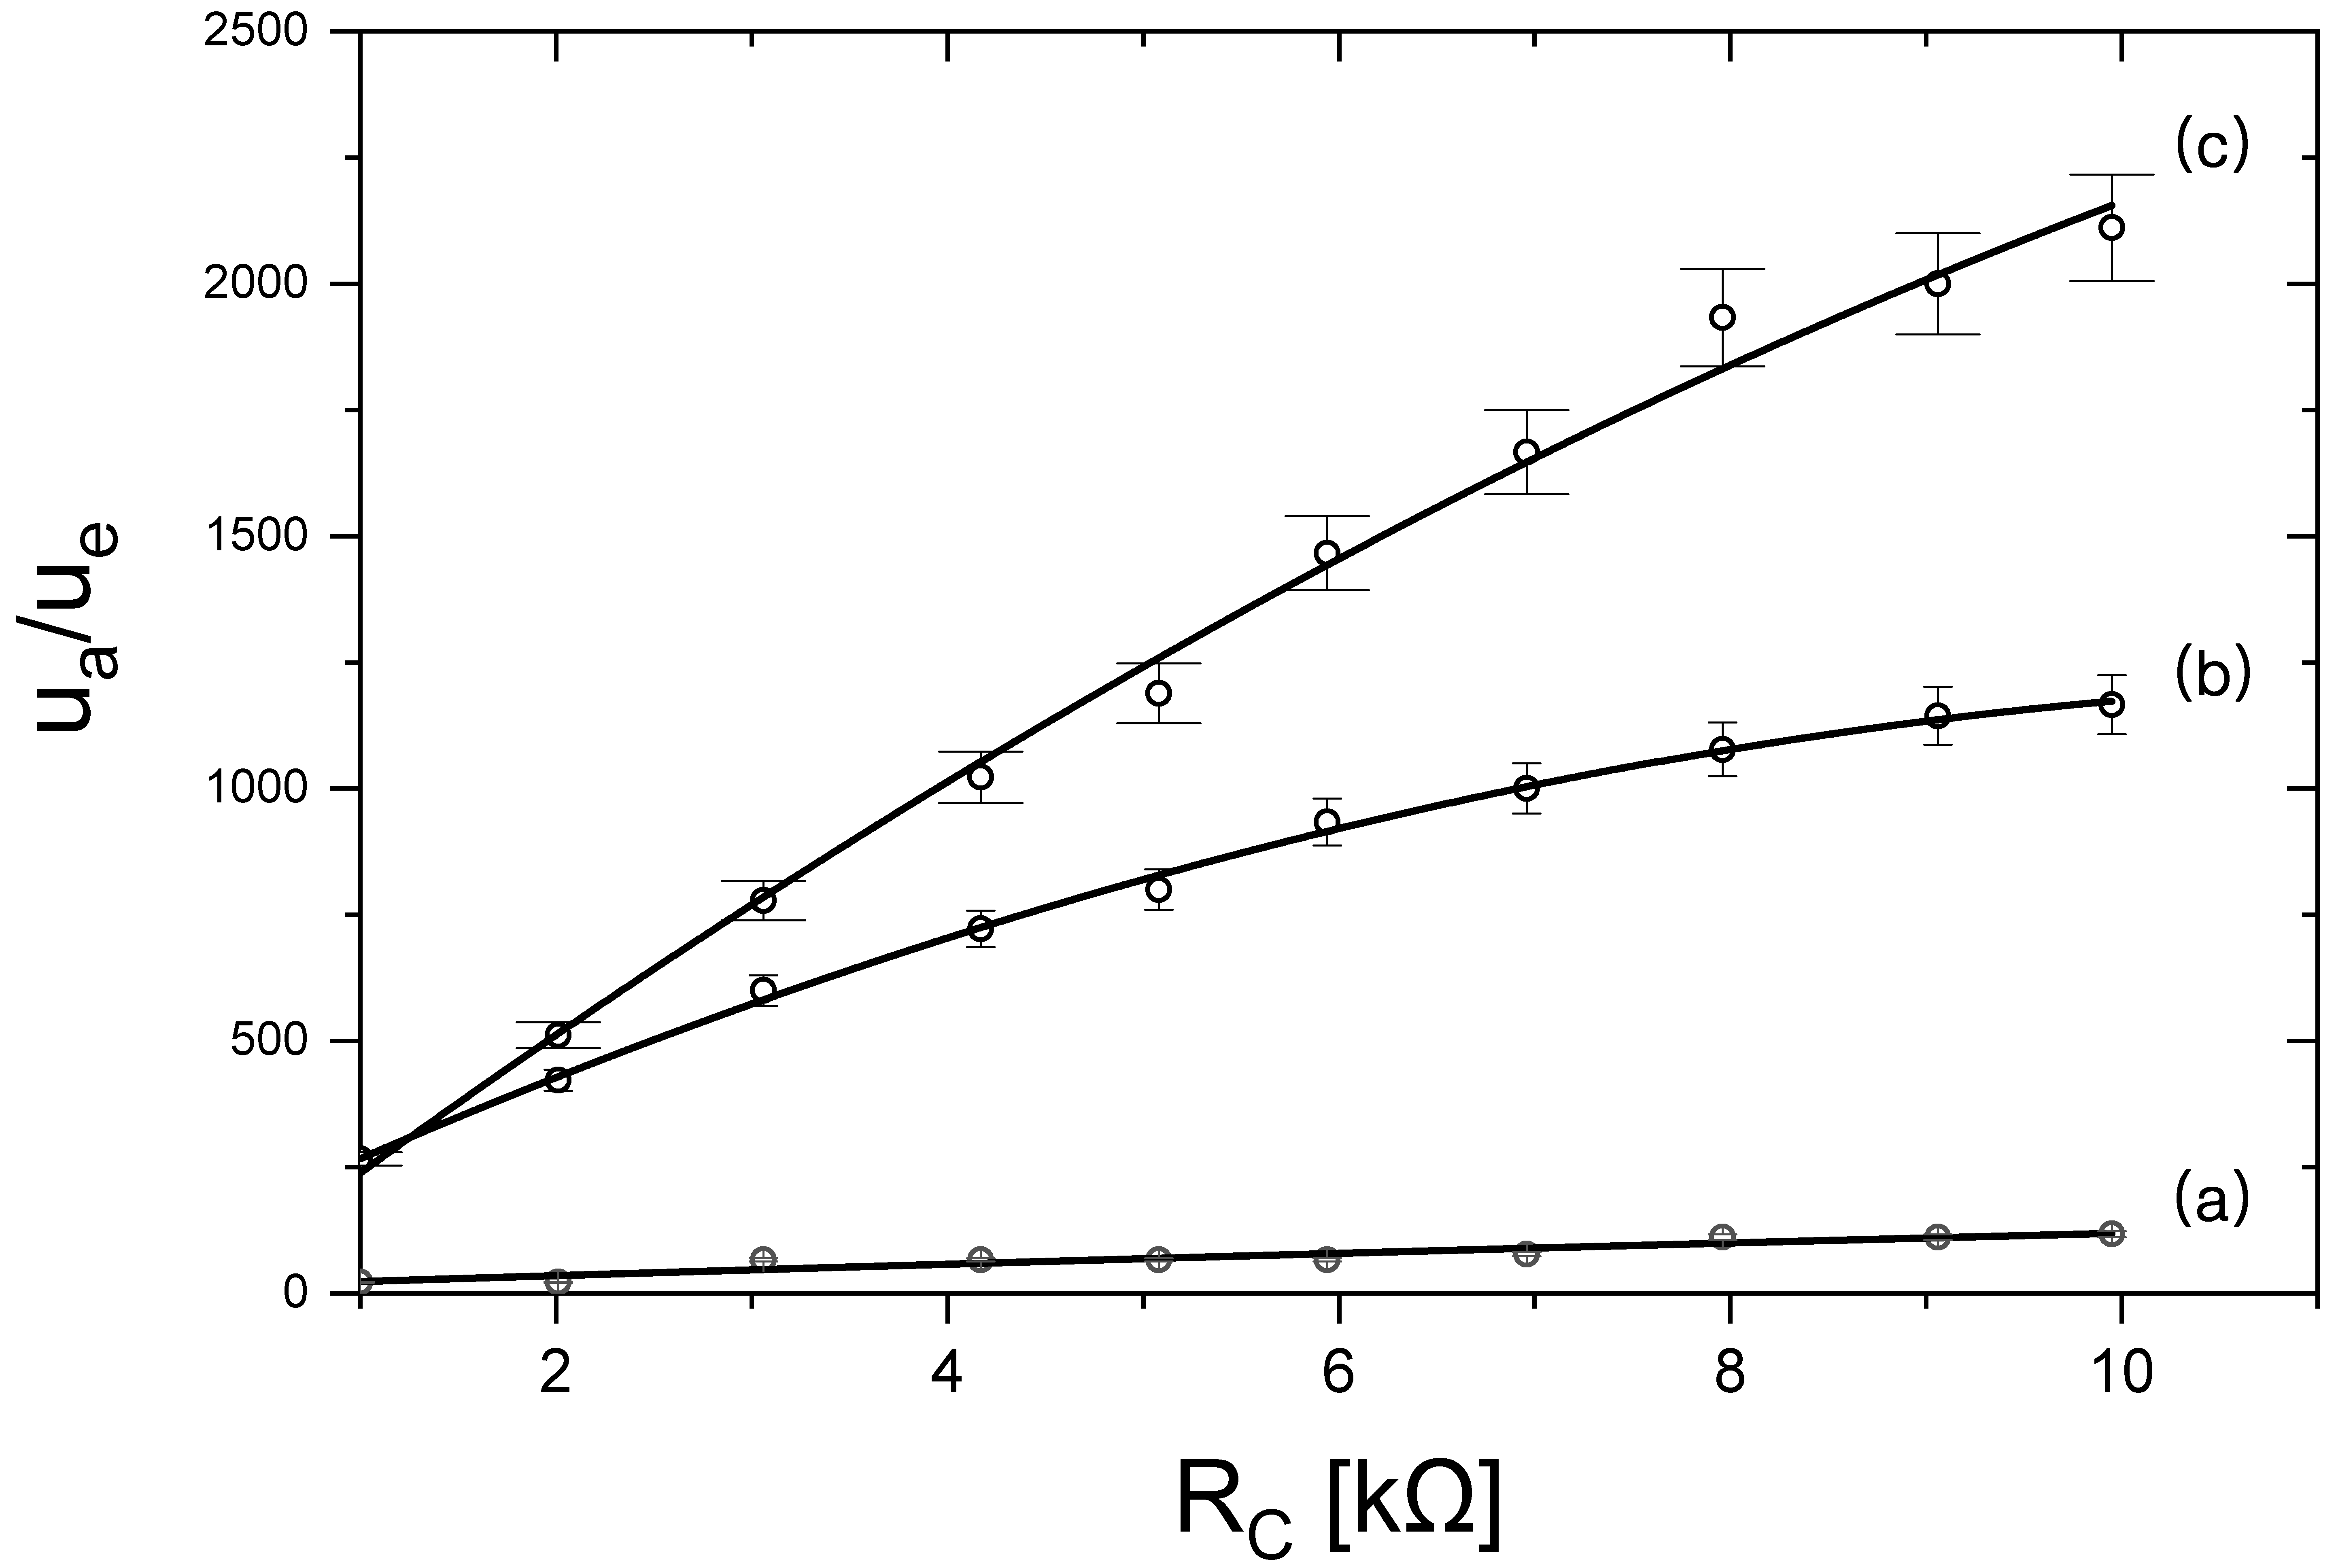
\includegraphics[width=140mm]{graphs/Verstrkung1.png}
                \caption{Verhältnis der Eingangs-zu Ausgangsamplitude $u_{\mathrm{a}} / u_{\mathrm{e}}$ von verschiedenen Konfigurationen. (a) Ohne Kondensator $C_E$ und ohne Lastwiderstand $R_L$, (b) mit Kondensator $C_E$ und Lastwiderstand $R_L=10$k$\Omega$, (c) mit Kondensator $C_E$ ohne Lastwiderstand $R_L$.}
                \label{fig:verstärkung}
            \end{figure*} \\
            % 2
            \noindent In Tabelle \ref{tab:verstärkung} sind die berechneten Werte der Verstärkung dargestellt. Bei Konfiguration (c) wurde ein Lastwiderstand von $R_L=10$k$\Omega$ gewählt. Für die Berechnung der Verstärkung musste zwischen Formel \ref{eq:A} und Formel \ref{eq:Aapprox} unterschieden werden. In Tabelle \ref{tab:verstärkung} wurde für (a) Formel \ref{eq:Aapprox} verwendet. Dabei wurde $R_L$ vernachlässigt, da dieser in der Konfiguration nicht vorhanden ist. Aus der Anleitung (\cite{anleitung}) ist die Wahl jedoch nicht klar, da die Konfiguartion der Schaltung ohne Lastwiderstand und ohne Kondensator nicht behandelt wird. Hierfür bot sich trotzdessen Formel \ref{eq:Aapprox} am besten an. Für Konfiguration (b) und (c) konnte Formel \ref{eq:A} verwendet werden. Dabei vereinfachte sich Formel \ref{eq:A} für (c) auf $A= -S \cdot R_C$. Bei Konfiguration (b) wurde Formel \ref{eq:A} zu $A=-S \cdot(\frac{1}{R_C} + \frac{1}{R_L})^{-1}$. Die Berechnung der Steilheit $S$ findet sich in Sektion \ref{subsec:Steil}.
            Die Verwendung der Formel für (b) und (c) geht direkt aus der Anleitung hervor. \\
            Eine weitere Diskussion der verschiedenen Konfiguration finde sich in Sektion \ref{sec:discussion} wieder.
        
            
            \begin{table}
                \centering
                \begin{tabular}{c|ccc}
                    \multicolumn{1}{c}{$R_C$ [k$\Omega$]} & \multicolumn{3}{c}{A} \\
                    \cmidrule(l){0-0}\cmidrule(lr){2-4}
                    \toprule
                         & (a)   & (b)     & (c)    \\ 
                    9.95 & -9.95 & -107.72 & -214.91  \\ 
                    9.06 & -9.06 & -102.67 & -195.69   \\ 
                    7.96 & -7.96 & -95.73 & -171.93   \\ 
                    6.96 & -6.96 & -88.64 & -150.33  \\
                    5.94 & -5.94 & -80.49 & -128.30 \\
                    5.08 & -5.08 & -72.76 & -109.72 \\
                    4.17 & -4.17   & -63.56   & -90.07 \\
                    3.06 & -3.06  & -50.60  & -66.09  \\
                    2.01 & -2.01 & -36.14 & -43.41  \\
                    0.99 & -0.99 & -19.45 & -21.38 \\
                    \bottomrule
                \end{tabular}
                \caption{Verstärkung der drei verschiedenen Konfigurationen. Hierbei handelt es sich um die selben Konfigurationen wie in Grafik \ref{fig:verstärkung}. Man beachte hierbei die kleinere Verstärkung gegenüber der in Grafik \ref{fig:verstärkung}, aufgrund der Verwendung des internen 10x-Tastteiler am Oszilloskop.}
                \label{tab:verstärkung}
            \end{table}
              
                
            
        \subsection{Frequenzgang}
            Bei der Verstärkung durch die Emitterspannung tritt nicht nur eine reine Spannungsverstärkung auf, sondern auch eine Phasenverschiebung vom Ausgangssignal $u_a$ gegenüber dem Eingangssignal $u_e$ auf. 
            
            \noindent Die Folgen der Emitterspannung in Bezug auf das Ausgangssignal $u_a$ sind in Grafik \ref{fig:freq} dargestellt.\\ 
            Man betrachte hierbei die Entstehung eines Plateaus. Für große Frequenzen bei $u_e$ verringert sich die Verstärkung von $u_e$. Dies ist in der fallenden Amplitude sichtbar. 
            
            % 1 
            \begin{figure*}
                \centering
                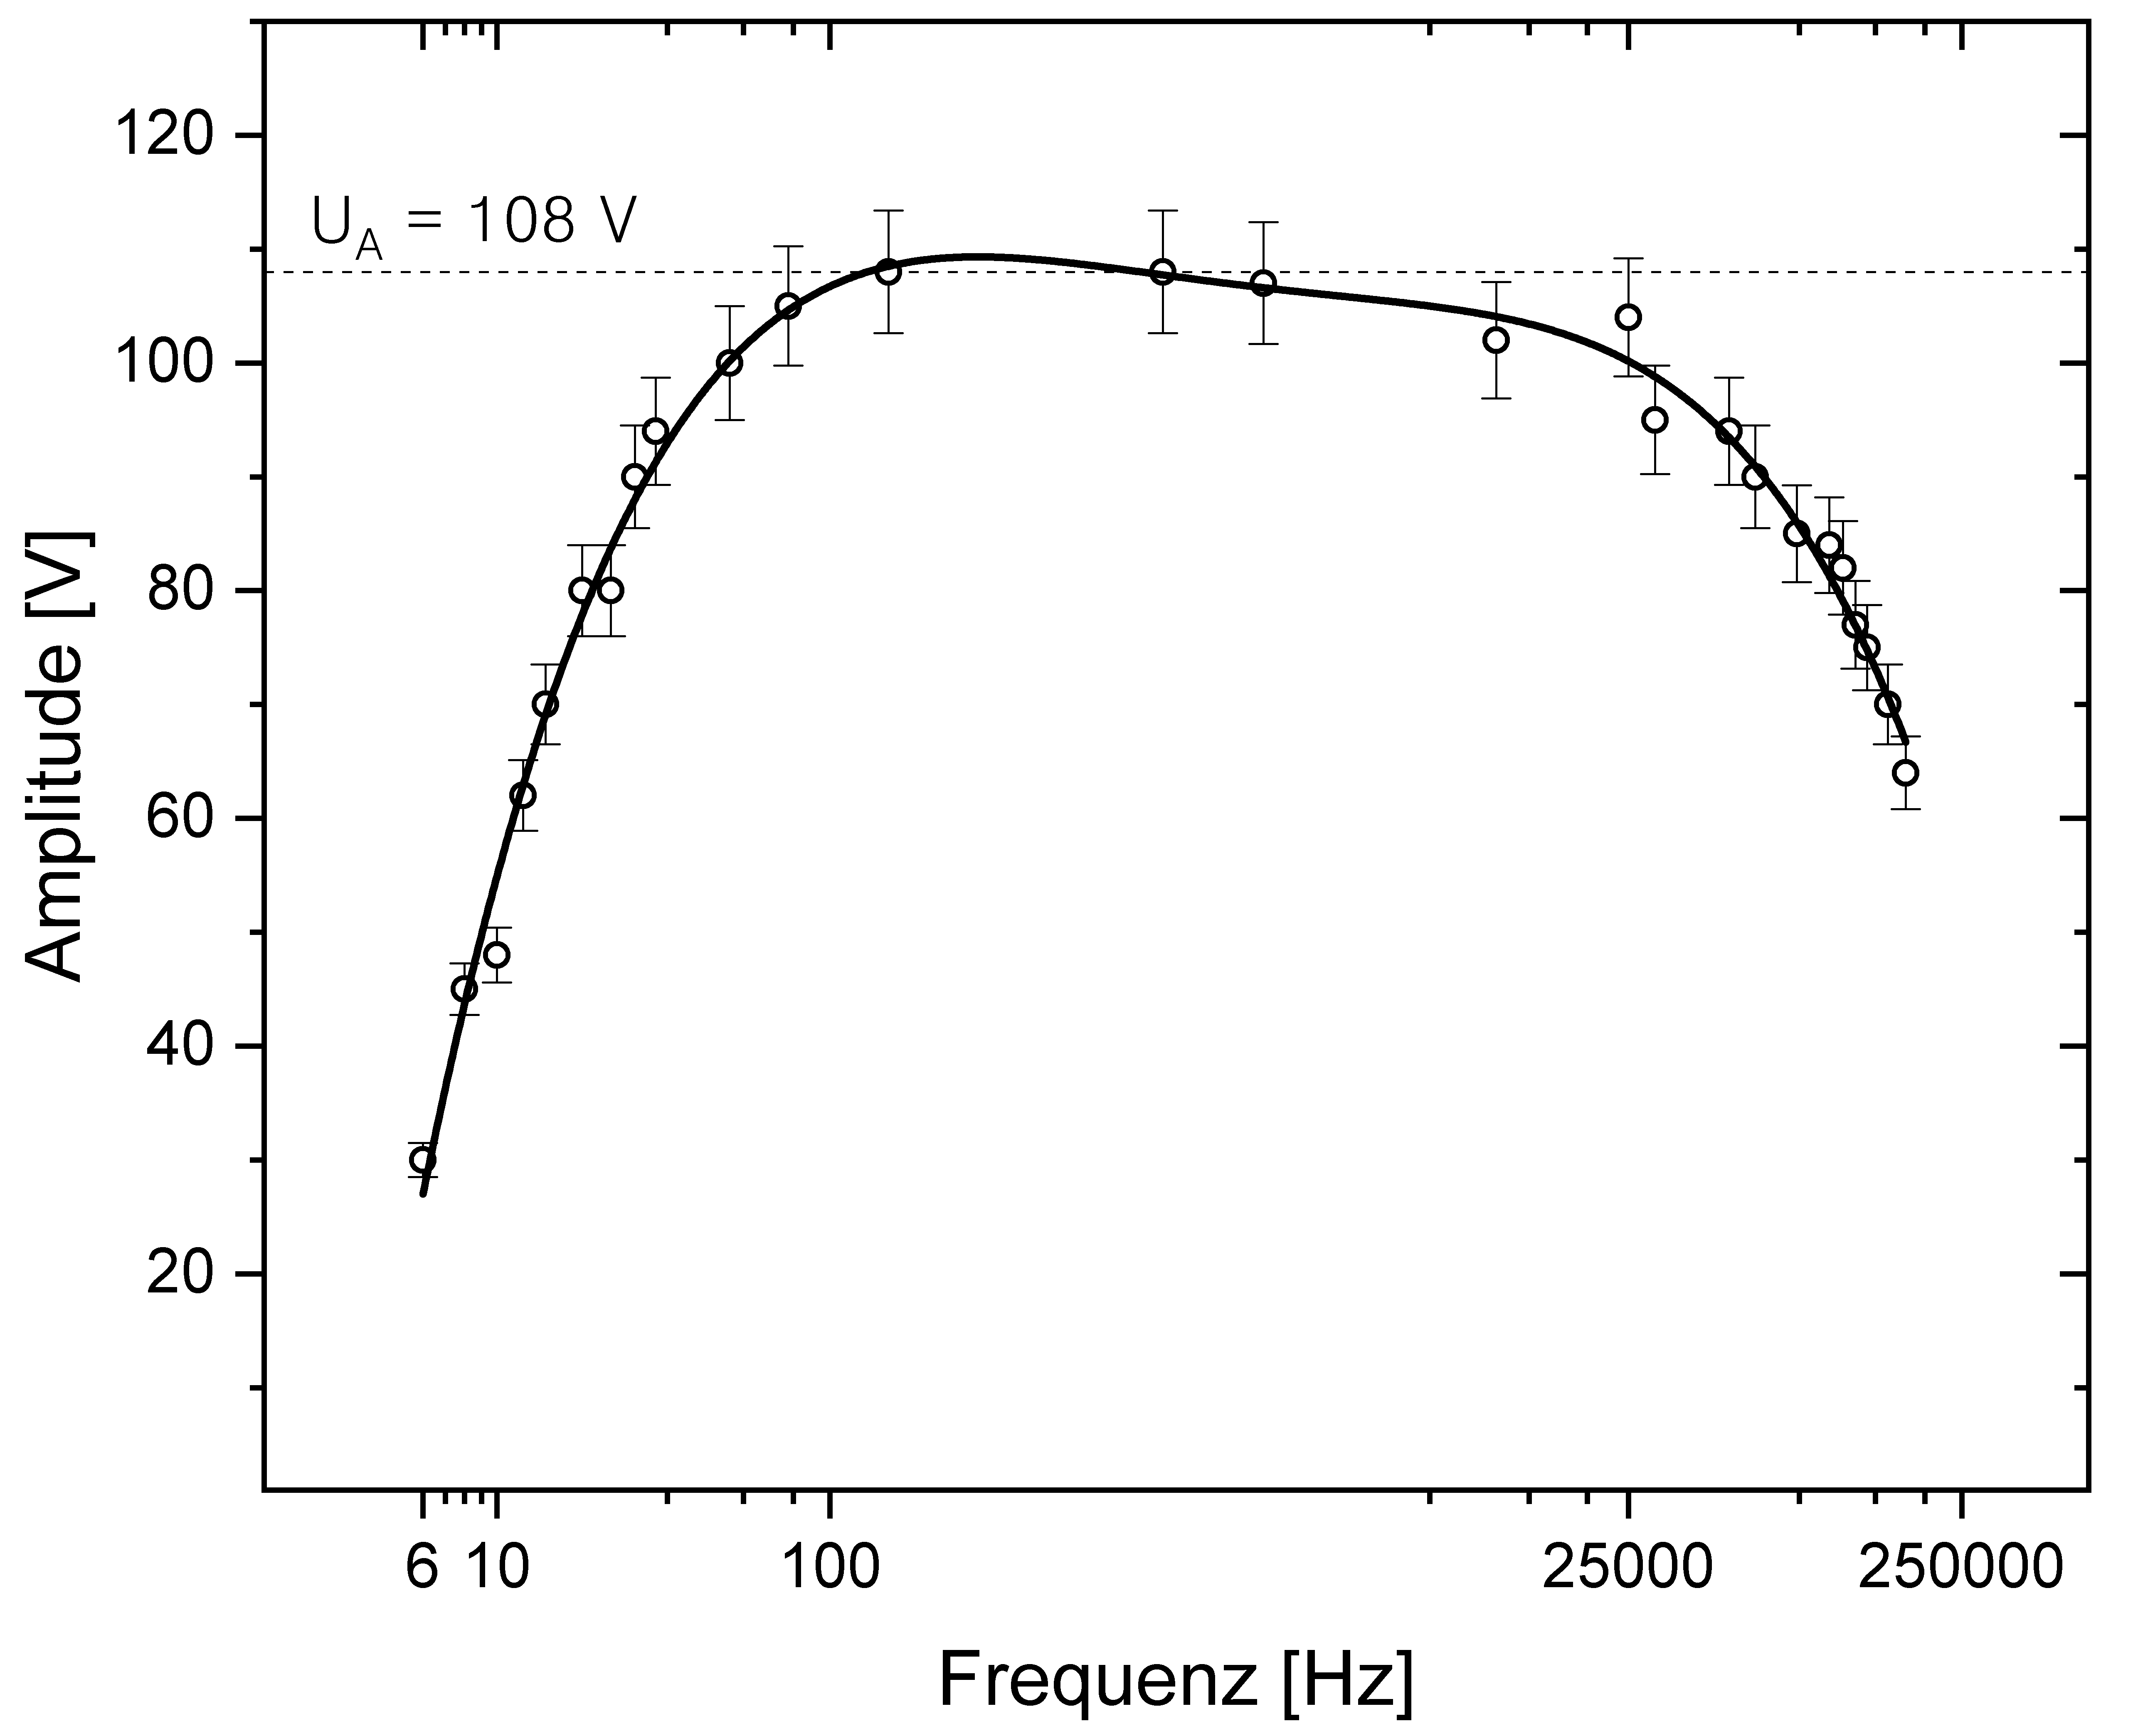
\includegraphics[width=78mm]{graphs/Frequenzgang1.png}
                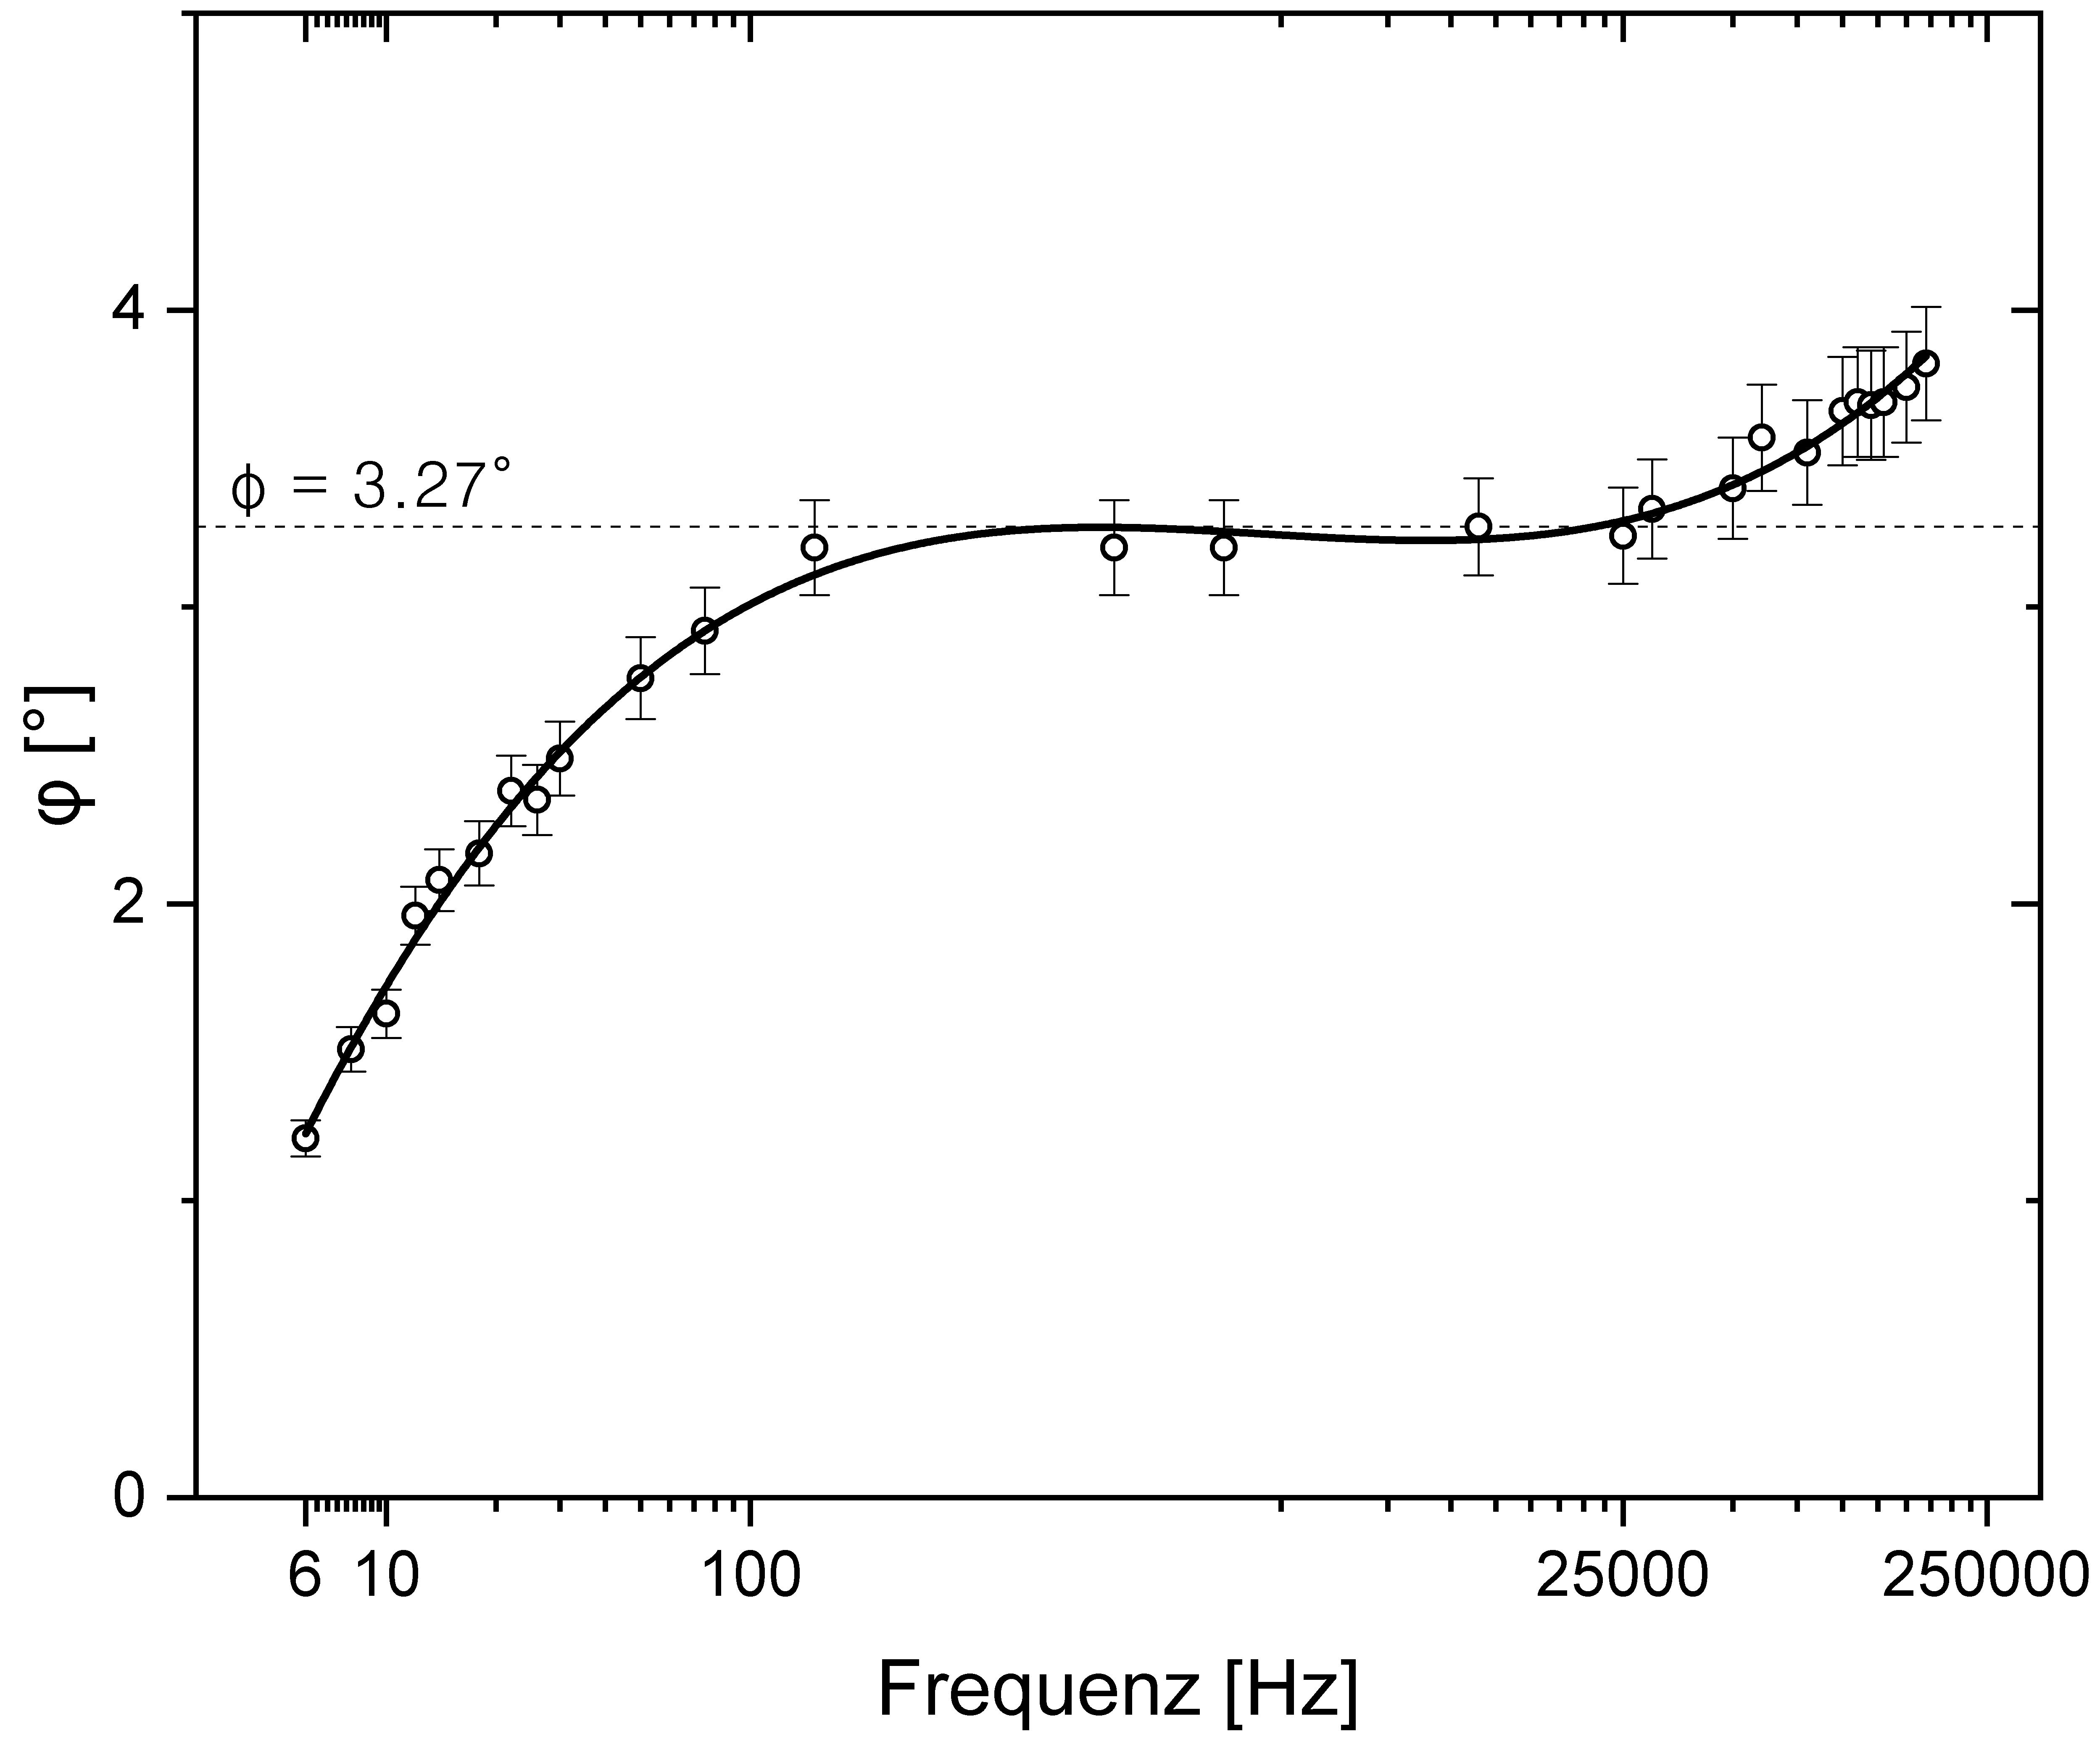
\includegraphics[width=78mm]{graphs/Frequenzgang2.png}
                \caption{Aplitudengang $A(f)$ (links) und Phasengang $\varphi(f)$ (rechts) mit dem jeweiligen eingezeichneten Plateau. Bei der Betrachtung des Plateaus, bei dem sich die Amplitude des Eingangssignal $u_e$ nicht ändert, fällt auf, dass auch der Phasenwinkel zwischen Eingangs- und Ausgangssignal sich nicht ändert. Das gemessene Plateau tritt für Frequenzen im Bereich von ungefähr [150, 25000] Hz auf. Man beachte die logarithmische x-Achse.}
                \label{fig:freq}
            \end{figure*}
            % 2
            \noindent Man betrachte $A(f)$ und $\varphi(f)$. Man erkennt, dass beide von 6Hz - 100Hz stark ansteigen. Darauf folgt das bereits genannte Plateau, bei dem sich beide Funktionen in erster Näherung nicht mehr ändern. Auf das Plateau folgt ein weiterer Bereich in dem sich die Funktionen ändern. Hierbei fällt die Amplitude von $u_a$ ab, wobei sich die Phasenverschiebung aber weiter fortsetzt. In Grafik \ref{fig:freq} sind die Änderungen nach dem Plateau proportional zu den Änderungen vor dem Plateau. Da die x-Achse jedoch logarithmisch skaliert ist, ist die Steigung der jeweiligen Funktion deutlich geringer.\\
            Eine weitere Betrachtung des Amplitudengangs der Emitterschaltung wirft deutliche Ähnlichenkeiten zu den Amplitudengangs eines Bandpassfilters auf. Hierbei verhält sich die Schaltung im Frequenzbereich von [6,100k]Hz wie ein Hochpass, im Frequenzbereich [100, 250]kHz wie ein Tiefpass. Da es auf dem Plateau keine Änderung der Amplitude gibt, bildet die Schaltung somit theoretisch sowhol einen Hoch- als auch Tiefpass.\\
            \\
            % 3 
            \textbf{Zwischen welchen Frequenzen findet man eine Verstärkung $|A| \geq \frac{1}{\sqrt{2}} \cdot\left|A_{\max }\right|$ vor?}\\
            Hierfür kann in Grafik \ref{fig:freq} bei $\frac{1}{\sqrt{2}} \cdot\left|A_{\max }\right|$ eine horizontale Linie gezogen werden. Bei $|A_{\max}|$ handelt es sich um die maximale Amplitude. Aus den gemessenen Werten ergibt sich somit für $|A_{\max}| \approx 108$V. Berechnung der Schnittpunkte der horizontalen Linie (bei U = 76.37V) mit der Amplitude von $u_a$, ergibt dies einen Frequenzbereich von etwa [50, 220000]Hz, in der die Ungleichung erfüllt ist.
            
            
            
        \subsection{Impedanzen von Übertragunsfunktionen von Hoch- und Tiefpass}
            Man betrachte die Schaltung in Abbildung \ref{fig:zweitor}. Für $\underline{I}_{\mathrm{a}}=0$ ergibt sich für diese die Übertragsfunktion
            
            \begin{equation}
                H\left(\underline{Z}_{1}, \underline{Z}_{2}\right)=\frac{\underline{U}_{\mathrm{a}}}{\underline{U}_{\mathrm{e}}} = \frac{Z_2}{Z_1+Z_2}
            \end{equation} \\
            Ebenso gilt die nachfolgende Matrixschreibweise.
             \begin{equation}
                \owncount
                \begin{pmatrix}
                    \underline{I}_e \\
                    \underline{I}_a
                \end{pmatrix}
                    =
                \begin{pmatrix}
                    \frac{1}{\underline{Z}_1} & -\frac{1}{\underline{Z}_1} \\
                    -\frac{1}{\underline{Z}_1} & \frac{1}{\underline{Z}_1} + \frac{1}{\underline{Z}_2}
                \end{pmatrix}
                \begin{pmatrix}
                    \underline{U}_e \\
                    \underline{U}_a
                \end{pmatrix} \\
                \label{eq:impd}
            \end{equation} \\
            Wählt man nun $\underline{Z}_{1} = C$ und $\underline{Z}_{2} = R$, so wird die Schaltung zu einem Hochpass. Die Übertragungsfunktion lautet dann wie folgt. 
            \begin{equation}
                \owncount
                H(j\omega) = \frac{R}{\frac{1}{iC\omega}+R}
            \end{equation} \\
            Setzt man $\underline{Z}_{2} = C$ und $\underline{Z}_{1} = R$, so wird die Schaltung zu einem Tiefpass mit der folgenden Übertragunsfunktion.
            \begin{equation}
                \owncount
                H(j\omega) = \frac{\frac{1}{iC\omega}}{\frac{1}{iC\omega}+R}
            \end{equation}
            
            \begin{figure}
                \centering
                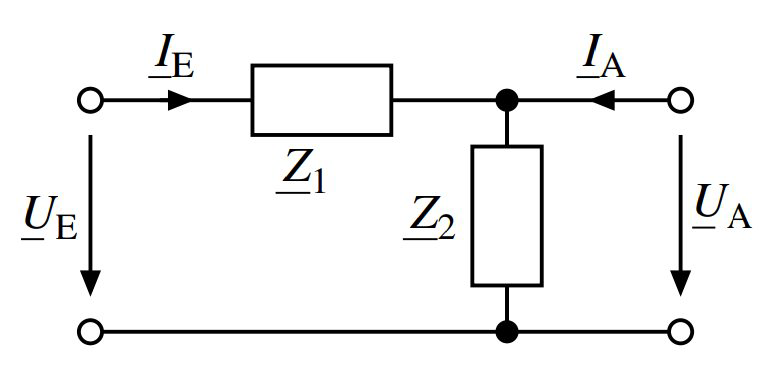
\includegraphics[width=50mm]{graphs/Zweitor.png}
                \caption{Einfaches Zweitor}
                \label{fig:zweitor}
            \end{figure}
            
            
    \section{Diskussion}\label{sec:discussion}
        Im folgenden werden die gemessenen Werte, wie sie in Sektion \ref{subsec:Versärkung} dargestellt wurde, genauer betrachtet und diskutiert. Es fällt auf, dass sich alle Schaltungen gleich verhalten. Das heißt bei zunehmenden Widerstand wirkt eine größere Verstärkung. Sie unterscheiden sich jedoch anhand ihres Maximalwertes. Der Maximalwert der Verstärkung für Schaltung (c) liegt bei etwa 2150, bei Schaltung (b) etwa 1100 und bei (c) etwa 10. Um diese Werte mit den Theoriewerten aus Tabelle \ref{tab:verstärkung} zu vergleichen, werden bei diesen der Betrag genommen. Es fällt auf, dass sich die Werte von (b) und (c) ähnlich zu den gemessen Werten verhalten. Sie unterscheiden sich um den Faktor 10, der aus der Tastteilereinstellung beim Oszilloskop folgt. Die Abflachung in (b) erscheint realistisch, da $R_L$ zu $R_C$ parallel geschalten worden ist. Auffällig ist jedoch das die Theoriewerte von (a) die selben Werte wie der eingestellte Widerstand haben. Da bei dieser Schaltung kein Kondensator mit eingebunden war konnte es zu keiner Rückkopplung kommen. Daher kommt es zu so gut wie keiner Verstäkung. 
      
    \section{Zusammenfassung}
        % TODO Wichtigste Punkte aufgreifen und zusammenfassen
        Damit ein Bipolartransistor in Emitterschaltung als Verstärker genutzt werden kann, muss unbedingt ein Kondensator zur Stromgegenkopplung eingebaut werden. Darüber hinaus wird die Verstärkung größer, je höher der Widerstand ist. Jedoch nur bis zu einem gewissen Sättigungsbereicht des Transistors. Der Transistor kann sich unter Betrieb erhitzen, was zu einer Arbeitspunktverschiebung führen würde. Da dies nicht erwünscht ist, wird ein zusätzliches Widerstand eingebaut.\\
        Die Funktionen des Transistors wird bei den Kennlienen noch einmal verdeutlicht. Bei der Eingangskennlinien wurde gezeigt, dass bei einer immer größer werdenden Spannung von $U_{BE}$ der Basisstorm $I_B$ rapide verstärkt wird. Bei der Ausgangskennlinie wurde gezeigt, dass bei einer kleinen angelegten Spannung $U_{CE}$ der Strom über den Kollektor $I_C$ rapide zunimmt. Ab einer gewissen Spannung vergrößert sich die Stromstärke nicht mehr, was den Stättigungsbereich des Transistors aufzeigt. 
        
        
        
        
    % References
    \bibliographystyle{mnras}
    \bibliography{Ausarbeitung.bib}
    


    % Appendix
    \appendix
    %\newpage
    \section{Fehlerrechnung}
    Die Fehlerrechnung betrachtet hier nur statistische Fehler. Sämtliche Werte, die Fehler beinhalten, wurden von Origin erstellt, bei dem angenommen wird, dass die Fehler des Programms rein statistischer Natur sind, oder von Messungsschwankungen des Multimeters stammen. Dessen Fehler wurde auf ein Digit geschätzt.
    Fehler für die Arbeitstemperatur:
    \begin{equation}
        \owncount
        \Delta T = \sqrt{(\frac{\Delta t_1}{t_1})^2} = 3,49K
    \end{equation}
    Fehler für die Steilheit S: 
    \begin{equation}
        \owncount
        \Delts S = \sqrt{(\frac{\Delta T}{T})^2 + (\frac{\Delta I_c}{I_C})^2} \cdot S = 0,21 \cdot 10^{-2} \frac{1}{\Omega}
    \end{equation} 
    
    
    
    % Don't change these lines
    \label{lastpage}
\end{document}
